\documentclass[border = 2mm]{standalone}
\usepackage[utf8]{inputenc}
\usepackage{tikz}
\usetikzlibrary{calc}

% Power of the outdoor station: panel -> charger -> battery, through the
% battery monitor, and charger -> Grove Shield. Every connector is drawn:
% sockets, plugs, solder joints, screw terminals and the lever connector.
% The thermistor is taped against the battery, and wired to the charger
% only.

\tikzset{
    module/.style={draw, thick, rounded corners=2pt, fill=#1, align=center,
        font=\sffamily\small, minimum height=1.2cm, minimum width=3cm},
    module/.default=gray!15,
    % JST-PH socket, fixed on a board (pins: "male")
    socket/.style={draw, thick, fill=white, minimum width=#1, minimum height=0.4cm,
        inner sep=0pt},
    socket/.default=0.8cm,
    % JST-PH plug, at the end of a cable (holes: "female")
    plug/.style={draw, thick, fill=gray!60, minimum width=#1, minimum height=0.5cm,
        inner sep=0pt},
    plug/.default=0.8cm,
    terminal/.style={draw, thick, fill=green!35, minimum size=0.45cm, inner sep=0pt},
    lever/.style={draw, thick, rounded corners=1pt, fill=orange!50,
        minimum width=1.1cm, minimum height=0.5cm, inner sep=0pt},
    label/.style={font=\sffamily\scriptsize, inner sep=1pt},
    wirePower/.style={red!80!black, very thick},
    wireGround/.style={black, very thick},
    wireI2c/.style={blue!70!black, very thick},
    wireNtc/.style={orange!80!black, thick},
    wirePanel/.style={gray!70!black, line width=2pt},
    note/.style={font=\sffamily\scriptsize, align=center},
}

% A solder joint
\newcommand{\solder}[1]{\fill (#1) circle (0.09)}
% A screw terminal: a square with its screw
\newcommand{\screwTerminal}[2]{%
    \node[terminal] (#1) at (#2) {};
    \draw (#2) circle (0.15);
    \draw ($(#2)+(-0.1,-0.1)$) -- ($(#2)+(0.1,0.1)$)}

\begin{document}
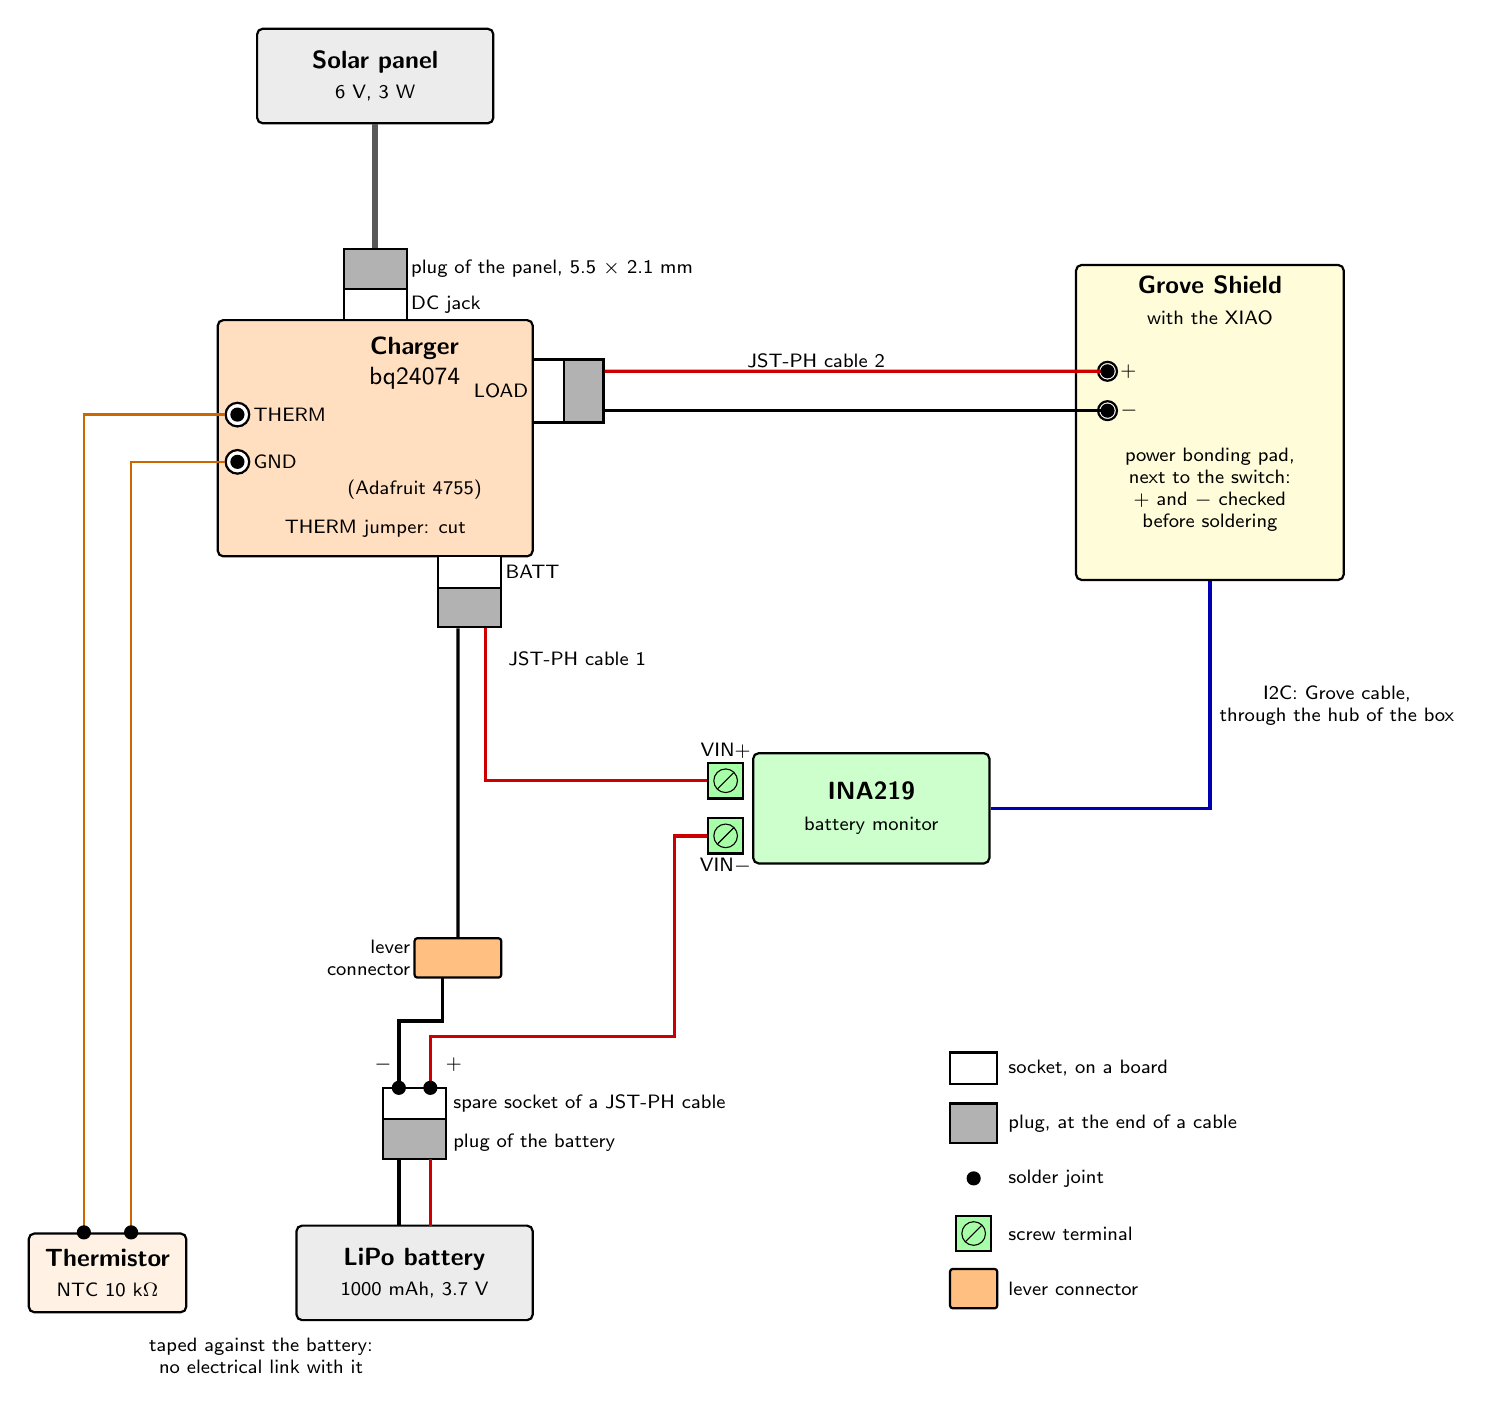
\begin{tikzpicture}

% ================================================================ modules
\node[module=gray!15] (panel) at (0,9.6) {\textbf{Solar panel}\\\scriptsize 6 V, 3 W};
\node[module=orange!25, minimum width=4cm, minimum height=3cm] (charger) at (0,5) {};
\node[font=\sffamily\small, align=center] at (0.5,5.95) {\textbf{Charger}\\bq24074};
\node[note] at (0.5,4.35) {(Adafruit 4755)};
\node[module=yellow!15, minimum width=3.4cm, minimum height=4cm] (shield) at (10.6,5.2) {};
\node[font=\sffamily\small, align=center] at (10.6,6.75) {\textbf{Grove Shield}\\\scriptsize with the XIAO};
\node[module=green!20, minimum height=1.4cm] (ina) at (6.3,0.3) {\textbf{INA219}\\\scriptsize battery monitor};
\node[module=gray!15] (battery) at (0.5,-5.6) {\textbf{LiPo battery}\\\scriptsize 1000 mAh, 3.7 V};
\node[module=orange!10, minimum width=2cm, minimum height=1cm] (ntc) at (-3.4,-5.6)
    {\textbf{Thermistor}\\\scriptsize NTC 10 k$\Omega$};

% ================================================================ panel -> charger
% DC jack of the charger, and the plug of the panel
\node[socket] (dcJack) at (0,6.7) {};
\node[plug] (dcPlug) at (0,7.15) {};
\node[label, right] at (dcJack.east) {DC jack};
\node[label, right] at (dcPlug.east) {plug of the panel, 5.5 $\times$ 2.1 mm};
\draw[wirePanel] (dcPlug.north) -- (panel.south);

% ================================================================ charger -> Grove Shield
% LOAD socket of the charger, and the plug of JST-PH cable 2
\node[socket=0.4cm, minimum height=0.8cm] (loadSocket) at (2.2,5.6) {};
\node[plug=0.5cm, minimum height=0.8cm] (loadPlug) at (2.65,5.6) {};
\node[label, left] at (loadSocket.west) {LOAD};
\node[label, above] at (5.6,5.85) {JST-PH cable 2};

% The two holes of the power bonding pad, next to the switch of the shield
\draw[thick, fill=white] (9.3,5.85) circle (0.12);
\draw[thick, fill=white] (9.3,5.35) circle (0.12);
\node[label, right] at (9.42,5.85) {+};
\node[label, right] at (9.42,5.35) {$-$};
\node[note, below] at (10.6,5.0) {power bonding pad,\\next to the switch:\\+ and $-$ checked\\before soldering};

\draw[wirePower] ($(loadPlug.east)+(0,0.25)$) -- (9.3,5.85);
\draw[wireGround] ($(loadPlug.east)+(0,-0.25)$) -- (9.3,5.35);
\solder{9.3,5.85};
\solder{9.3,5.35};

% ================================================================ charger -> INA219 -> battery
% BATT socket of the charger, and the plug of JST-PH cable 1
\node[socket] (battSocket) at (1.2,3.3) {};
\node[plug] (battPlug) at (1.2,2.85) {};
\node[label, right] at (battSocket.east) {BATT};
\node[label, right] at (1.65,2.2) {JST-PH cable 1};

% Screw terminals of the INA219
\screwTerminal{vinPlus}{4.45,0.65};
\screwTerminal{vinMinus}{4.45,-0.05};
\node[label, above] at (vinPlus.north) {VIN+};
\node[label, below] at (vinMinus.south) {VIN$-$};

% Lever connector: joins the two - wires
\node[lever] (lever) at (1.05,-1.6) {};
\node[label, left, align=right] at (lever.west) {lever\\connector};

% Cable 1: red to VIN+, black to the lever connector
\draw[wirePower] ($(battPlug.south)+(0.2,0)$) |- (vinPlus.west);
\draw[wireGround] ($(battPlug.south)+(-0.15,0)$) -- (lever.north);

% The spare socket, with two wires soldered to its pins, receives the
% plug of the battery: its + goes to VIN-, its - to the lever connector
\node[socket] (spareSocket) at (0.5,-3.45) {};
\node[plug] (batteryPlug) at (0.5,-3.9) {};
\node[label, right] at (0.95,-3.45) {spare socket of a JST-PH cable};
\node[label, right] at (0.95,-3.95) {plug of the battery};
\draw[wirePower] (0.7,-3.25) |- (3.8,-2.6) |- (vinMinus.west);
\draw[wireGround] (0.3,-3.25) |- (0.85,-2.4) -- (0.85,-1.85);
\solder{0.7,-3.25};
\solder{0.3,-3.25};
\node[label, left] at (0.25,-2.95) {$-$};
\node[label] at (1.0,-2.95) {+};
% The short leads of the battery, up to its plug
\draw[wirePower] (0.7,-4.15) -- (0.7,-5.0);
\draw[wireGround] (0.3,-4.15) -- (0.3,-5.0);

% INA219 -> board, on the I2C bus
\draw[wireI2c] (ina.east) -| (shield.south);
\node[note, right] at (10.6,1.6) {I2C: Grove cable,\\through the hub of the box};

% ================================================================ thermistor
% Two pins of the header of the charger, side by side: THERM and GND
\node[draw, thick, fill=white, circle, minimum size=0.3cm, inner sep=0pt] (thermPin) at (-1.75,5.3) {};
\node[draw, thick, fill=white, circle, minimum size=0.3cm, inner sep=0pt] (gndPin) at (-1.75,4.7) {};
\node[label, right] at (thermPin.east) {THERM};
\node[label, right] at (gndPin.east) {GND};
\node[note] at (0,3.85) {THERM jumper: cut};

\draw[wireNtc] ($(ntc.north)+(-0.3,0)$) |- (thermPin.west);
\draw[wireNtc] ($(ntc.north)+(0.3,0)$) |- (gndPin.west);
\solder{thermPin.center};
\solder{gndPin.center};
\solder{$(ntc.north)+(-0.3,0)$};
\solder{$(ntc.north)+(0.3,0)$};
% Taped against the cell: a thermal contact, not an electrical one
\node[note, below] at (-1.45,-6.3) {taped against the battery:\\no electrical link with it};

% ================================================================ legend
\begin{scope}[shift={(7.6,-3.0)}]
    \node[socket=0.6cm] at (0,0) {};
    \node[label, right] at (0.4,0) {socket, on a board};
    \node[plug=0.6cm] at (0,-0.7) {};
    \node[label, right] at (0.4,-0.7) {plug, at the end of a cable};
    \solder{0,-1.4};
    \node[label, right] at (0.4,-1.4) {solder joint};
    \screwTerminal{legendTerminal}{0,-2.1};
    \node[label, right] at (0.4,-2.1) {screw terminal};
    \node[lever, minimum width=0.6cm] at (0,-2.8) {};
    \node[label, right] at (0.4,-2.8) {lever connector};
\end{scope}

\end{tikzpicture}
\end{document}
